\documentclass{article}
\usepackage[utf8]{inputenc}
\usepackage{amsmath,amsthm,amssymb}
\usepackage[dutch]{babel}
\usepackage{float}
\usepackage{longtable}
\usepackage[margin=2cm]{geometry}
\usepackage{graphicx}
\usepackage{color}
\usepackage{xcolor}
\usepackage{hyperref}
\usepackage{algorithm}
\usepackage{algorithmic}
\usepackage[labelfont=bf,justification=centering]{caption}

\begin{document}
\begin{titlepage}
	
	\newcommand{\HRule}{\rule{\linewidth}{0.5mm}}
	
	\center
	
	\textsc{\LARGE Katholieke Universiteit Leuven}\\[1.5cm]
	\textsc{\Large Bachelor informatica}\\[0.5cm]
	\textsc{\large Toepassingen van de meetkunde in de informatica}\\[0.5cm]
	
	\HRule \\[0.4cm]
	{ \huge \bfseries Practicum\\ Snijdende rechthoeken }\\[0.4cm]
	\HRule \\[1.5cm]
	\begin{minipage}
		{0.4
		\textwidth} 
		\begin{flushleft}
		    \large \emph{Door:}\\
			Alexandra \textsc{Kolchedantseva} \\
			\emph{r0478263}\\
			\large \emph{en}\\
			Mathias \textsc{Van Herreweghe} \\
			\emph{r0456156}
		\end{flushleft}
	\end{minipage}
	~ 
	\begin{minipage}
		{0.4
		\textwidth} 
		\begin{flushright}
			\large \emph{In opdracht van:} \\
			Professor \\
			Dirk \textsc{Roose} 
		\end{flushright}
	\end{minipage}
	\\[4cm]
	
	{\large Academiejaar 2015 - 2016}\\
	\begin{figure}
		[b] \centering 
		
\includegraphics[scale = 0.2]{kul.png} 
	\end{figure}
\end{titlepage}

\tableofcontents
\newpage
\section{Inleiding}
We zullen in dit verslag een klein onderzoek doen naar het berekenen van snijpunten bij rechthoeken. De keuze van programmeertaal was vrij, hiervoor hebben wij gekozen voor Java aangezien we hier het meeste ervaring mee hebben.

Het verslag behandelt drie algoritmen, met een verschillende tijdscomplexiteit. We beginnen met een na\"ief algoritme en werken onze weg omhoog naar een complexer algoritme met verscheidene optimalisaties.

Concreet zullen we een algemene beschrijving in woorden geven van de algoritmen, alsook voorzien we de code op hoogniveau. Verder leiden we de tijdscomplexiteit van deze algoritmen af. Daarnaast zullen we experimenten doen met verschillende waarden voor de maximum zijde van een algoritme, ook zullen we de correctheid van onze algoritmen praktisch aantonen. 

Ten slotte geven we nog een bemerking mee die we ondervonden tijdens het maken van het practicum.



\newpage
\section{De verschillende algoritmen}





\subsection{Berekenen van de snijpunten}
\subsubsection{Beschrijving}
In de methode \texttt{getIntersections} worden er twee rechthoeken meegegeven. Eerst wordt er met behulp van de methode \texttt{overlaps} gekeken of de twee gegeven rechthoeken overlappen. Als dit niet het geval is wordt een lege lijst teruggegeven. 
Anders gaan we verder met het algoritme. We berekenen eerst de rechthoek \texttt{rechthoek1} $\cap$ \texttt{rechthoek2}. 
\begin{itemize}
\item De x-co\"ordinaat van de linkeronderhoek van deze rechthoek is gelijk aan het maximum van de x-co\"ordinaat van de linkeronderhoek van \texttt{rechthoek1} en die van \texttt{rechthoek2}. 
\item De x-co\"ordinaat van de rechterbovenhoek van deze rechthoek is gelijk aan het minimum van de x-co\"ordinaat van de rechterbovenhoek van \texttt{rechthoek1} en die van \texttt{rechthoek2}.
\item De y-co\"ordinaat van de linkeronderhoek van deze rechthoek is gelijk aan het maximum van de y-co\"ordinaat van de linkeronderhoek van \texttt{rechthoek1} en die van \texttt{rechthoek2}.
\item De y-co\"ordinaat van de rechterbovenhoek van deze rechthoek is gelijk aan het minimum van de y-co\"ordinaat van de rechterbovenhoek van \texttt{rechthoek1} en die van \texttt{rechthoek2}.
\end{itemize}

Alle hoekpunten van de bekomen rechthoeken voegen we toe aan een lijst met mogelijk intersectiepunten. Voor elk van deze punten gaan we na of dat dit punt zowel een element is van \texttt{rechthoek1} als van \texttt{rechthoek2}, deze controle noemen we \texttt{isIntersectionWithBoth}. Daarna wordt er gecontroleerd of dat deze punten wel degelijk \emph{snij}-punten zijn, met andere woorden mag een punt dat een element is van beide rechthoeken niet snijden op dezelfde as. We noemen deze controle \texttt{isIntersectOnIdenticalAxis}. Als \texttt{isIntersectionWithBoth} slaagt en \texttt{isIntersectOnIdenticalAxis} faalt, is het een geldig punt en slaagt \texttt{isValidIntersect} bijgevolg. We geven nu een korte beschrijving van deze controles in psueodocode.

\begin{algorithm}
\caption{Controle of een gegeven punt een geldig snijpunt is}
\begin{algorithmic}[1]
	\STATE \textbf{Input:}  $punt$: een punt met x- en y-co\"ordinaat. $r1$: rechthoek1. $r2$= rechthoek2. \COMMENT{elke rechthoek bevat een linkeronderhoek en rechterbovenhoek, aangegeven met $rX.leftBottom$ en $rX.rightTop$.}
	\STATE $isIntersectionWithR1 =$ (punt.x == r1.leftBottom.x) \OR (punt.x == r1.rightTop.x) \OR (punt.y == r1.leftBottom.y) \OR (punt.y == r1.rightTop.y)
	\STATE $isIntersectionWithR2 =$ (punt.x == r2.leftBottom.x) \OR (punt.x == r2.rightTop.x) \OR (punt.y == r2.leftBottom.y) \OR (punt.y == r2.rightTop.y)
	\STATE $isIntersectionWithBoth = isIntersectionWithR1$ \AND $isIntersectionWithR2$
	
	\STATE $intersectsOnIdenticalX$ = ((punt.x == r1.leftBottom.x) \AND (punt.x == r2.leftBottom.x)) \OR ((punt.x == r1.rightTop.x) \AND (punt.x == r2.rightTop.x));
	\STATE $intersectsOnIdenticalY$ = ((punt.y == r1.leftBottom.y) \AND (punt.y == r2.leftBottom.y)) \OR ((punt.y == r1.rightTop.y) \AND (punt.y == r2.rightTop.y));
	\STATE $isIntersectionOnIdenticalAxis$ = $intersectsOnIdenticalX$ \OR $intersectsOnIdenticalY$
	\STATE $isValidIntersect$ = $isIntersectionWithBoth$ \AND \NOT$intersectOnIdenticalAxis$
	\RETURN $isValidIntersect$
\end{algorithmic}
\end{algorithm}

Met behulp van deze controles worden praktisch alle uitzonderlijkheden of randgevallen in rekening gebracht. Dit is met uitzondering van geroteerde rechthoeken uiteraard, maar dit ligt buiten het bereik van dit practicum.
Hierbij is eveneens de correctheid van het bepalen van snijpunten van twee gegeven rechthoeken aangetoond.

\subsubsection{Complexiteit}
Het berekenen van de snijpunten van twee rechthoeken gebeurt in constante uitvoeringstijd. Door op voorhand na te gaan (in een nog lagere constante uitvoeringstijd) of twee rechthoeken wel degelijk snijden gebeurt dit gemiddeld gezien sneller dan zonder deze controle.




\newpage
\subsection{Algoritme 1}
\label{algo1_1}
\subsubsection{Algemeen}
Dit algoritme vergelijkt elke rechthoek \'e\'en keer met elke andere rechthoek. Er wordt in \texttt{getIntersections} nagegaan of twee rechthoeken snijden, indien dit het geval is worden de snijpunten berekend en teruggegeven.

\subsubsection{Hoogniveau beschrijving}
\label{algo1_2}
\begin{algorithm}
\caption{Bereken alle snijpunten van een verzameling rechthoeken}
\begin{algorithmic}
	\STATE \textbf{Input:}  $rechthoeken$: Een lijst met $n$ rechthoeken
	\STATE $snijpunten$ $\gets \emptyset$
    \FOR{$i = 0 \to n-1$}
       \FOR{$j = i+1 \to n-1$} 
            \STATE  voeg getIntersections($rechthoeken$[i], $rechthoeken$[j]) toe bij $snijpunten$
        \ENDFOR
    \ENDFOR
    \RETURN{$snijpunten$}
\end{algorithmic}
\end{algorithm}

\subsubsection{Complexiteit}
\label{algo1_3}
Er zijn $N$ rechthoeken gegeven, voor de eerste rechthoek worden er dus $(N-1)$ rechthoeken gecontroleerd, voor de volgende $(N-2)$ enzoverder. Uiteindelijk bekomen we dus

\[ (N-1) + (N-2) + \dots + 1 = \frac{N \cdot (N-1)}{2}\]
controles van rechthoeken. Bijgevolg is de tijdscomplexiteit $\mathcal{O}(n^2)$.


\subsubsection{Correctheid}
\begin{proof} eindigheid.\\
Het algoritme eindigt. De instructie in de binnenste for-lus
wordt namelijk exact \[\sum_{i=1}^{n} \sum_{j=i+1}^{n} 1 = \frac{n(n-1)}{2} \]
keer uitgevoerd.
\end{proof}

\begin{proof} correctheid.\\
We vergelijken elke rechthoek met elke andere rechthoek. Aangezien we reeds aangetoond hebben dat het berekenen van snijpunten van twee rechthoeken correct is, is algoritme 1 bijgevolg ook correct.
\end{proof}


\newpage
\subsection{Algoritme 2}
\subsubsection{Algemeen}
\label{algo2_1}
In dit algoritme wordt met een doorlooplijn gewerkt. Deze doorlooplijn doorloopt het veld van links naar rechts en voegt telkens een rechthoek toe aan een lijst van actieve rechthoeken wanneer het het meest linkse punt van die rechthoek aantreft, deze rechthoek wordt terug verwijderd als tijdens de uitvoering van het algoritme het meest rechtste punt van deze rechthoek aantreft. Al deze actieve rechthoeken worden gesorteerd van klein naar groot op basis van de $x$-co\"ordinaat (vandaar dat het algoritme van links naar rechts werkt).
Bij het tegenkomen van een nieuwe rechthoek zal het algoritme controleren of deze rechthoek snijdt met een of meerdere actieve rechthoeken. Rechthoeken die niet bij de actieve rechthoeken horen kunnen onmogelijk snijden met de huidige rechthoek aangezien men een rechte kan trekken tussen de twee rechthoeken om ze zo te scheiden in verschillende secties.


\subsubsection{Hoogniveau beschrijving}
\label{algo2_2}
\begin{algorithm}
\caption{Bereken alle snijpunten van een verzameling rechthoeken met behulp van een doorlooplijnalgoritme}
\begin{algorithmic}
	\STATE \textbf{Input:}  $rechthoeken$: Lijst met $n$ rechthoeken
	\STATE $snijpunten$ $\gets \emptyset$
	\STATE $eenheden$: Lijst met uiterst links en rechtse x-co\"ordinaat van elke rechthoek, gesorteerd op x-waarde
	\STATE $actieveRechthoeken$ $\gets \emptyset$ (Een set die de actieve rechthoeken bevat)
    \FORALL{$eenheid$ in $eenheden$}
        \IF{$eenheid$ is linker $x$-co\"ordinaat van $eenheid.rechthoek$}
            \FORALL{$actieveRechthoek$ in $actieveRechthoeken$}
                 \STATE  voeg getIntersections($eenheid.rechthoek$, $actieveRechthoek$) toe bij $snijpunten$
            \ENDFOR
            \STATE voeg $eenheid.rechthoek$ toe bij $actieveRechthoeken$
        \ELSE
        \STATE verwijder $eenheid.rechthoek$ van $actieveRechthoeken$
        \ENDIF
    \ENDFOR
    \RETURN $snijpunten$
\end{algorithmic}
\end{algorithm}

\newpage
\subsubsection{Complexiteit}
\label{algo2_3}
De complexiteit wordt opnieuw gecontroleerd op basis van het aantal controles op snijpunten tussen twee rechthoeken. Deze controle gebeurt nu enkel bij het tegenkomen van een links punt van een rechthoek, er zijn dan $N$ controles uit de lijst van $2\cdot N$ elementen, met $N$ het aantal gegeven rechthoeken. Op het moment van een controle worden er $X$ controles gedaan met $X$ het aantal actieve rechthoeken. In het slechtste geval zijn alle gegeven rechthoeken actief en is $X = N$ en zal elke rechthoek dus gecontroleerd moeten worden. In dit (worst case) scenario bekomen we dus net zoals in \ref{algo1_3}
\[ \frac{N \cdot (N-1)}{2}\]
vergelijkingen aangezien er nooit een rechthoek verwijderd wordt uit de actieve rechthoeken. We bekomen dus bijgevolg in het slechtste geval dus opnieuw $\mathcal{O}(n^2)$. We visualiseren dit probleem met onderstaande afbeelding waar men kan zien dat een rechthoek (voorgesteld door een lijn ter verduidelijking) pas zal verwijderd worden op het einde van het algoritme.


\begin{figure}[H]
\centering
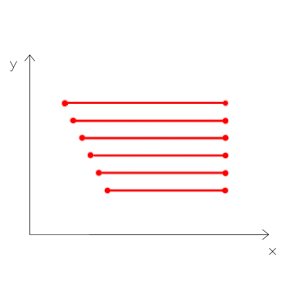
\includegraphics[width=6cm,height=6cm,keepaspectratio]{algo2_problem}
\caption{Verduidelijking van de worst case bij algoritme 2.}
\end{figure}

\subsubsection{Correctheid}
\label{algo2_4}
Aangezien er niet expliciet gevraagd wordt voor een correctheidsbewijs voor elk algoritme, vertrekken we vanuit de bewezen correctheid van algoritme 1. Omdat algoritme 1 bewezen is, kunnen we er met ruim voldoende zekerheid vanuit gaan dat als algoritme 2 steeds dezelfde snijpunten geeft als algoritme 1, algoritme 2 correct is bij het nagaan van bij 100 test-cases opbouwend van 50 rechthoeken tot en met 5000 met telkens 50 meer rechthoeken dan voorheen, en voor elke testcase (dus voor elk bepaald aantal rechthoeken) doen we de test vijfmaal met verschillende willekeurig gegenereerde rechthoeken.
Na het uitvoeren van deze test bevatten de uitkomsten van beide algoritmen exact dezelfde snijpunten, weliswaar in een andere volgorde, bijgevolg is algoritme 2 correct.

\newpage
\subsection{Algoritme 3}
\subsubsection{Algemeen}
\label{algo3_1}
Algoritme 3 is gelijkaardig aan algoritme 2. Algoritme 3 gebruikt echter een binaire zoekboom (BST) om de actieve rechthoeken en de reikwijdtes bij te houden. De BST van de actieve rechthoeken wordt gesorteerd op basis van de $y$-co\"ordinaat van het middelpunt (sleutel) van een rechthoek en bevat als waarde de actieve rechthoek. De BST van de reikwijdtes is gesorteerd op basis van de reikwijdte (sleutel), en bevat als waarde het aantal actieve voorkomens van deze reikwijdte. Het bijhouden van het actief aantal voorkomens van deze reikwijdtes is noodzakelijk om te voorkomen dat een reikwijdte uit de BST wordt verwijderd terwijl er nog een andere actieve rechthoek is die een evengrote reikwijdte heeft.

De doorlooplijn van het algoritme werkt nog steeds van links naar rechts. In plaats van de huidige rechthoek met elke actieve rechthoek uit het segment te vergelijken zoals bij het algoritme 2, wordt nu alleen vergeleken met rechthoeken die binnen de -tot dan toe grootste tegengekomen- reikwijdte ligt van de huidige rechthoek. Concreet worden enkel de actieve rechthoeken beschouwd met een $y$-co\"ordinaat van hun middelpunt die ligt tussen hun laagste waarde op de $y$-as afgetrokken met de maximum reikwijdte, en hun hoogste waarde op de $y$-as opgeteld met de maximum reikwijdte. Zo wordt er vermeden dat rechthoeken worden gecontroleerd die buiten het bereik liggen. Deze maximum reikwijdte wordt steeds up-to-date gehouden bij het toevoegen en verwijderen van actieve rechthoeken.

\subsubsection{Hoogniveau beschrijving}
\label{algo3_2}
\begin{algorithm}[H]
\caption{Bereken alle snijpunten van een verzameling rechthoeken met behulp van een doorlooplijnalgoritme en een binaire zoekboom}
\begin{algorithmic}
	\STATE \textbf{Input:}  $rechthoeken$: Een lijst met $n$ rechthoeken
	\STATE $snijpunten$ $\gets \emptyset$
	\STATE $eenheden$: Lijst met uiterst links en rechtse x-co\"ordinaat van elke rechthoek, gesorteerd op x-waarde
	\STATE $queue$ $\gets \emptyset$ (Binaire zoekboom met actieve rechthoeken, gesorteerd op de $y$-co\"ordinaat van middelpunt)
	\STATE $reikwijdtes$ $\gets \emptyset$ (Een binaire zoekboom die als sleutel de reikwijdtes van actieve rechthoeken bevat, met reikwijdte $=$ hoogte rechthoek $/2$, en als waarde het aantal voorkomens van deze reikwijdte)
	\STATE $maxReikwijdte \gets 0$ (houdt de grootste reikwijdte van de actieve rechthoeken bij)
    \FORALL{$eenheid$ in $eenheden$}
        \STATE $huidigeReikwijdte =$ eenheid.rechthoek.hoogte $/2$
        \IF{$eenheid$ is linker $x$-co\"ordinaat van $eenheid.rechthoek$}
            \STATE $ondergrens =$ ($y$-co\"ordinaat van linkeronderhoek van $eenheid.rechthoek$) $- maxReikwijdte$
            \STATE $bovengrens =$ ($y$-co\"ordinaat van rechterbovenhoek van $eenheid.rechthoek$) $+ maxReikwijdte$
            \FORALL{$actieveRechthoek$ in deelverzameling van $queue$ betreffende de rechthoeken met $y$-co\"ordinaat van middelpunt tussen $ondergrens$ en $bovengrens$}
                 \STATE  voeg getIntersections($eenheid.rechthoek$, $actieveRechthoek$) toe bij $snijpunten$
            \ENDFOR
            \STATE voeg $eenheid.rechthoek$ met sleutel ($y$-co\"ordinaat van diens middelpunt) toe aan $queue$
            \STATE $maxReikwijdte =$ maximum van $maxReikwijdte$ en $huidigeReikwijdte$
            \IF{$reikwijdtes$ bevat $huidigeReikwijdte$}
                \STATE voeg $huidigeReikwijdte$ met als aantal ($huidigeReikwijdte.aantal$ + 1) toe aan $reikwijdtes$
            \ELSE
                \STATE voeg $huidigeReikwijdte$ met als aantal 1 toe aan $reikwijdtes$
            \ENDIF
        \ELSE
            \STATE verwijder het element met sleutel de $y$-co\"ordinaat van het middelpunt van $eenheid.rechthoek$
            \IF{$huidigeReikwijdte$ met aantal > 1 keer in $reikwijdtes$}
                \STATE voeg $huidigeReikwijdte$ met als aantal ($huidigeReikwijdte.aantal$ - 1) toe aan $reikwijdtes$
            \ELSE
                \STATE verwijder $huidigeReikwijdte$ van $reikwijdtes$
            \ENDIF
            \STATE $maxReikwijdte = 0$ als $reikwijdtes$ leeg is, anders gelijk aan element met de max sleutel van $reikwijdtes$
        \ENDIF
    \ENDFOR
    \RETURN $snijpunten$
\end{algorithmic}
\end{algorithm}

\subsubsection{Complexiteit}
\label{algo3_3}
De complexiteit van dit algoritme is een goede benadering voor de gevraagde complexiteit $\mathcal{O}((N+S)\log_2(N))$ in de opgave, met $S$ het aantal snijpunten. Er zullen namelijk onnodige (onsuccesvolle) controles uitgevoerd worden op een aantal rechthoeken die binnen de reikwijdte liggen maar desondanks niet snijden, dit probleem verduidelijken we in onderstaande figuur.

\begin{figure}[H]
\centering
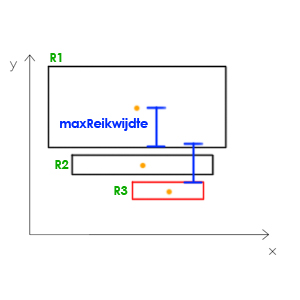
\includegraphics[width=8cm,height=8cm,keepaspectratio]{algo3_problem}
\caption{Verduidelijking van onnodige controles bij algoritme 3.}\label{algo3_problem}
\end{figure}

Zoals we in de figuur zien, is de reikwijdte van rechthoek 1 (aangeduid met \texttt{\textbf{{\color{green}R1}}}) de maximum reikwijdte onder de actieve rechthoeken. Bij het tegenkomen van rechthoek 3 tijdens het doorlooplijnalgoritme ligt rechthoek 2 binnen het te controleren interval op de $y$-as. Vooral bij het voorkomen van erg grote rechthoeken zou dit dus een groot probleem kunnen zijn, aangezien de max reikwijdte dan heel groot is en er dus meer kans is dat andere actieve rechthoeken binnen het te controleren interval liggen.

Bij het berekenen van de complexiteit bouwen we voort op het kwadratische uitvoeringstijd (in het slechtste geval) van sectie \ref{algo2_3}. Het verschil is dat we nu minder rechthoeken onnodig zullen controleren op snijpunten met een huidige rechthoek. Het nagaan welke rechthoeken binnen het te controleren interval liggen kost in de door ons gebruikte (ongebalanceerde) binaire zoekboom $\mathcal{O}(N)$ tijd. We gaan ervan uit dat de BST gemiddeld verdeeld is en bijgevolg een complexiteit heeft van $\mathcal{O}(K\cdot\log_2(N))$ met K het gevonden aantal. 

Wel moeten we vermelden dat in het slechtste geval nog steeds alle rechthoeken worden gecontroleerd wat een complexiteit zou geven van $\mathcal{O}(N\cdot(N\cdot\log_2(N))=\mathcal{O}(N^2\cdot\log_2(N))$. Ook de \texttt{contains} methode in de BST gebruikt $\mathcal{O}(\log_2(N))$ tijd, maar aangezien dit een optelling wordt met de vorige bekomen tijd kunnen we dit laten vallen per definitie van de Big-Oh notatie. Dit geldt eveneens voor het toevoegen en verwijderen van elementen bij de BST.

Verder merken we op dat hoe groter het aantal snijpunten, hoe groter de uitvoeringstijd. Het aantal rechthoeken in de binnenste lus dat wordt nagegekeken, dus de overlappende rechthoeken, noemen we R. Het aantal keer dat twee rechthoeken snijden ($=S$) is dan $\mathcal{O}(R)$, met andere woorden is S dus van grootteorde R.
Zo bekomen we uiteindelijk de complexiteit
\[\mathcal{O}(N\cdot(S+\log_2 N)).\]

\subsubsection{Correctheid}
De correctheid tonen we aan op een volledig analoge manier als in sectie \ref{algo2_4}.
Aangezien er niet expliciet gevraagd wordt voor een correctheidsbewijs voor elk algoritme, vertrekken we vanuit de bewezen correctheid van algoritme 1. Omdat algoritme 1 bewezen is, kunnen we er met ruim voldoende zekerheid vanuit gaan dat als algoritme 3 steeds dezelfde snijpunten geeft als algoritme 1, algoritme 3 correct is bij het nagaan van bij 100 test-cases opbouwend van 50 rechthoeken tot en met 5000 met telkens 50 meer rechthoeken dan voorheen, en voor elke testcase (dus voor elk bepaald aantal rechthoeken) doen we de test vijfmaal met verschillende willekeurig gegenereerde rechthoeken.
Na het uitvoeren van deze test bevatten de uitkomsten van beide algoritmen exact dezelfde snijpunten, weliswaar in een andere volgorde, bijgevolg is algoritme 3 correct.

\newpage
\section{Experimenten}
\begin{figure}[H]
\label{fig-exp}
\centering
\includegraphics[width=6cm,height=6cm,keepaspectratio]{{Experiment0.02}.png}
\includegraphics[width=6cm,height=6cm,keepaspectratio]{{Experiment0.2}.png}
\includegraphics[width=6cm,height=6cm,keepaspectratio]{{Experiment0.4}.png}
\includegraphics[width=6cm,height=6cm,keepaspectratio]{{Experiment0.8}.png}
\caption{Uitvoeringstijden bij rechthoeken met maximale zijde van $0.02$, $0.2$, $0.4$ en $0.8$.}
\end{figure}

De eerste plot die het gebruik van  een zeer kleine maximum zijde van $0.02$ visualiseert, laat duidelijk het verschil in tijdscomplexiteit zien. We zien het kwadratisch verloop van algoritme 1 en merken op dat algoritme 3 sneller presteert dan algoritme 2.

In de tweede plot van de figuur zien we dezelfde verhouding tussen de verschillende algoritmen. Daarnaast is in deze plot ook duidelijk dat algoritme 3 de berekende tijdscomplexiteit $\mathcal{O}(N\cdot(S+\log_2 N))$ volgt. Verder zien we dat algoritme 2 tussen de best case tijdscomplexiteit $\mathcal{O}(N\cdot\log_2(N))$ en de worst case tijdscomplexiteit van $\mathcal{O}(N^2)$ ligt. Deze neight duidelijk bij een een kleine maximum zijde (en dus relatief weinig snijdingen) naar de best case dan de worst case.

Bij de derde plot die gebruik maakt van de maximum zijde $0.4$ -wat toch al behoorlijk groot is op het interval $[0,1]$- valt er meteen iets op. Door het relatief hoog aantal snijdingen krijgen de optimalisaties van algoritme 2 en 3 weinig kans om minder rechthoeken te beschouwen dan algoritme 1. Bijgevolg neigen algoritme 2 en 3 eerder naar hun worst case tijdscomplexiteit dan hun gemiddelde tijdscomplexiteit.

In de vierde plot trekt de lijn zich voort vanuit de vorige plot, algoritme 2 en 3 gedragen zich erg gelijkaardig aan algoritme 1 wat betreft tijdscomplexiteit. Door het hoog aantal snijdingen zien we duidelijk dat de worst case tijdscomplexiteit van algoritme 3 ($\mathcal{O}(N^2\cdot\log_2(N))$ zelfs slechter is dan die van algoritme 1 en 2. Vooral bij een groot aantal rechthoeken ($>4000$) is deze trend duidelijk zichtbaar. Daarnaast valt het op dat bij dergelijk aantal snijpunten ten gevolge van de maximum zijde van $0.8$ de tijd benodigd voor het berekenen van die snijpunten gemiddeld al rond de 3900 milliseconden of bijna 4 seconden ligt bij algoritme 3. Dit is meer dan dubbel zoveel als algoritme 1 en 2 nodig hebben. Wederom is dit te wijten aan het feit bijna alle rechthoeken voor elke rechthoek met gecontroleerd worden op snijpunten, zoals uitgelegd in sectie \ref{algo2_3} en gevisualiseerd in figuur \ref{algo3_problem}.

\newpage
\section{Bemerkingen}
In de opgave werd aangehaald dat we een (ongebalanceerde) binaire zoekboom konden gebruiken voor onze implementatie, meer specifiek \url{http://algs4.cs.princeton.edu/32bst/BST.java.html} voor Java. Het gebruik van deze zoekboom belet ons de gevraagde tijdscomplexiteit van $\mathcal{O}((N+S)\cdot\log_2(N))$ te bekomen bij algoritme 3. Dit komt doordat we een opzoeking doen (namelijk \texttt{keys}) die gemiddeld tijdscomplexiteit $\mathcal{O}(K\cdot\log_2(N))$ heeft met K een constante, en zelfs $\mathcal{O}(N)$ in het slechtste geval.
Het gebruik van een boom die beter bij de noden van onze algoritmen past zoals een \textit{balanced binary searchtree}, \textit{segment searchtree}, \textit{interval searchtree} of een \textit{range searchtree} zouden allemaal leiden tot de gevraagde tijdscomplexiteit. Dit omdat de opvraging vergelijkbaar met \texttt{keys} uit de BST bij deze bomen maar $\mathcal{O}(K+\log_2(N))$ in beslag neemt, met K het aantal gevonden objecten. Desondanks zou dit dezelfde worst case tijdscomplexiteit geven voor algoritme 3. Wel moeten we opmerken dat het gebruik van deze bomen onze algoritmen aanzienlijk complexer zou kunnen maken door de wijze waarop deze zoekbomen zijn opgebouwd.
\end{document}
